
%-------------------------------------------------------------------------------
%							THIRD SECTION
%-------------------------------------------------------------------------------



\section{\textsc{Travaux et résultats}}


\subsection{Résultats en 1D}

\begin{frame}{Déplacement des noeuds d’un floe isolé (1)}

    \mycols{

        \mycol{50}{
            \myfigframe{Deplacement1D-Systeme.png}{Floe de glace 1D}

            \begin{figure}[!h]
                \begin{subfigure}[b]{0.47\textwidth}
                    \centering
                    \frame{\includegraphics[width=\textwidth]{Deplacement1D-Masse1.png}}
                    % \caption{Sur la masse $m$ de gauche.}
                \end{subfigure}
                \begin{subfigure}[b]{0.43\textwidth}
                    \centering
                    \frame{\includegraphics[width=\textwidth]{Deplacement1D-Masse2.png}}
                    % \caption{Sur la masse $m$ de droite.}
                \end{subfigure}
                   \caption{Bilan des forces}
            \end{figure}
        }

        \mycol{50}{
            Les équations de Newton-Euler:
            \begin{align*}
                \begin{dcases}
                m\ddot x_1 = - k(x_1 - x_2) - \mu(\dot x_1 - \dot x_2) \,,\\
                    m \ddot x_2 =  k(x_1 - x_2) + \mu(\dot x_1 - \dot x_2) \,. 
                \end{dcases}
            \end{align*}

            On préfère la forme générique:
            \begin{align*}
                \begin{dcases}
                    \dot{Y}(t)= E Y(t) \,,\\
                    Y_0 = Y(0) = (0,0,v_0,-v'_0)^T \,,
                \end{dcases}
            \end{align*}

            où :
            \begin{align*}
                E = \begin{pmatrix}
                    0 & 0 & 1 & 0 \\ 0 & 0& 0& 1 \\ -\frac{k}{m} & \frac{k}{m} & -\frac{\mu}{m} & \frac{\mu}{m} \\ \frac{k}{m} & -\frac{k}{m} & \frac{\mu}{m} & -\frac{\mu}{m}
                \end{pmatrix} \,,
                \text{ et } Y = \begin{pmatrix} x_1 \\ x_2 \\ \dot{x}_1 \\ \dot{x}_2 \end{pmatrix} 
            \end{align*}
        }
    }

    \note{Ici, ne pas utiliser un repère absolu, on peut utiliser un qui soit relatif au floe. Dans ce cas, on a convergence.}
    
\end{frame}


\begin{frame}[fragile]{Déplacement des noeuds d’un floe isolé (2)}

    \begin{columns}[onlytextwidth]

        \begin{column}{0.5\textwidth}
            \begin{lstlisting}[language=Python,caption=Code de simulation avec Scipy]
    Y0 = np.array([0,0, v0, -v_0])
    t = np.linspace(0, tmax, N+1)
    def model(Y, t):
        return E @ Y
    Y = odeint(model, Y0, t)
            \end{lstlisting}
        \end{column}

        \mycol{50}{    
        \begin{theorem}[Convergence du modèle 1D isolé]
            Les déplacements $x_1$ et $x_2$ des noeuds du floe 1D convergent si et seulement si leurs vitesses initiales sont des vecteurs opposés.
        \end{theorem}
        }
    \end{columns}
    

    
    \begin{figure}[!h]
        \centering
        \begin{subfigure}[t]{0.45\textwidth}
            \centering
            \includegraphics[width=\textwidth]{SimuDeplacement1D1.png}
            \caption{$v_0=v'_0 = 0.8$}
        \end{subfigure}
        \begin{subfigure}[t]{0.45\textwidth}
            \centering
            \includegraphics[width=\textwidth]{SimuDeplacement1D2.png}
            \caption{$v_0= 0.6$ et $v'_0 = 0.8$}
        \end{subfigure}    
        \caption{Simulation du déplacement d'un floe en 1D}
    \end{figure}

\end{frame}




\begin{frame}{Collision parfaitement inélastique avec un floe encastré à l’instant initial}

    \mycols{

        \mycol{55}{
            \myfigframe{Percussion1D-Systeme}{Collision 1D avec fixation d'un floe}

            \begin{figure}[!h]
                \begin{subfigure}[b]{0.54\textwidth}
                    \centering
                    \frame{\includegraphics[width=\textwidth]{Percussion1D-Masse1}}
                \end{subfigure}
                \begin{subfigure}[b]{0.435\textwidth}
                    \centering
                    \frame{\includegraphics[width=\textwidth]{Percussion1D-Masse2}}
                \end{subfigure}
                   \caption{Bilan des forces}
            \end{figure}

            Le système est régi par les équations :
            \begin{align*}
                \begin{dcases}
                (m+m')\ddot x_1 = -kx_1 - \mu \dot x_1 + k'(x_2 - x_1) + \mu'(\dot x_2 - \dot x_1) \\
                    m' \ddot x_2 =  -k'(x_2 - x_1) - \mu'(\dot x_2 - \dot x_1) 
                \end{dcases}
            \end{align*}

        }

        \mycol{45}{

            \myfig{SimuPercussion1D.png}{Résultat de simulation}
        }

    }
    
\end{frame}


\begin{frame}{Collision parfaitement inélastique sans présence du mur}

    \mycols{

        \mycol{55}{
            \myfigframe{Percussion1D-Systeme-2}{Collision 1D sans mur}

            \begin{figure}[!h]
                \begin{subfigure}[b]{0.30\textwidth}
                    \centering
                    \frame{\includegraphics[width=\textwidth]{Percussion1D2-Masse1.png}}
                \end{subfigure}
                \begin{subfigure}[b]{0.38\textwidth}
                    \centering
                    \frame{\includegraphics[width=\textwidth]{Percussion1D2-Masse2}}
                \end{subfigure}
                \begin{subfigure}[b]{0.26\textwidth}
                    \centering
                    \frame{\includegraphics[width=\textwidth]{Percussion1D2-Masse3}}
                \end{subfigure}
                   \caption{Bilan des forces}
            \end{figure}

            Le système est régi par les équations :
            \begin{align*}
                \begin{dcases}
                m\ddot x_1 = -k(x_1 - x_2) - \mu (\dot x_1 - \dot x_2) \,, \\
                (m+m')\ddot x_2 = k(x_1 - x_2) + \mu (\dot x_1 - \dot x_2) - k'(x_2 - x_3) - \mu'(\dot x_2 - \dot x_3) \,, \\
                    m' \ddot x_3 =  k'(x_2 - x_3) + \mu'(\dot x_2 - \dot x_3) \,. 
                \end{dcases}
            \end{align*}

        }

        \mycol{45}{
            % \myfig{SimuPercussion1D2.png}{Résultat de simulation}

            \vspace*{-0.25cm}

            \begin{figure}[!h]
                \begin{subfigure}[t]{\textwidth}
                    \centering
                    \includegraphics[width=0.9\textwidth]{SimuPercussion1D2.png}
                    \caption{Cas convergent}
                \end{subfigure}
                \begin{subfigure}[t]{\textwidth}
                    \centering
                    \includegraphics[width=0.9\textwidth]{SimuPercussion1D2NonConv.png}
                    \caption{Cas non convergent}
                \end{subfigure}
                   \caption{Résultat de simulation}
            \end{figure}

            \begin{alertblock}{Note}
                Critère de convergence pas clair!
            \end{alertblock}

        }

    }
    
\end{frame}


\begin{frame}{Collision inélastique avec séparation des masses (1)}

    \mycols{

        \mycol{50}{
            \myfigframe{Percussion1D-Systeme-3}{Collision 1D inélastique}

            \vspace*{-0.5cm}
            \begin{figure}[!h]
                \begin{subfigure}[b]{0.35\textwidth}
                    \centering
                    \frame{\includegraphics[width=\textwidth]{Percussion1D3-Masse1.png}}
                \end{subfigure}
            %     \hfill
                \begin{subfigure}[b]{0.48\textwidth}
                    \centering
                    \frame{\includegraphics[width=\textwidth]{Percussion1D3-Masse2}}
                \end{subfigure}
            %     \hfill
                \begin{subfigure}[b]{0.44\textwidth}
                    \centering
                    \frame{\includegraphics[width=\textwidth]{Percussion1D3-Masse3}}
                \end{subfigure}
            %     \hfill
                \begin{subfigure}[b]{0.35\textwidth}
                    \centering
                    \frame{\includegraphics[width=\textwidth]{Percussion1D3-Masse4}}
                \end{subfigure}
                   \caption{Bilan des forces}
            \end{figure}

            \vspace*{-0.5cm}
            \myfigframe{Percussion1D3-Apres.png}{Situation \alert{après} contact}

        }

        \mycol{50}{
            Le système est régi par les équations :
            \begin{align*}
                \begin{dcases}
                m\ddot x_1 = -k(x_1 - x_2) - \mu (\dot x_1 - \dot x_2) \,, \\
                m\ddot x_2 = k(x_1 - x_2) + \mu (\dot x_1 - \dot x_2) - \alert{F_c} \,, \\
                m'\ddot x_3 = - k'(x_3 - x_4) - \mu'(\dot x_3 - \dot x_4) + \alert{F_c} \,, \\
                    m' \ddot x_4 =  k'(x_3 - x_4) + \mu'(\dot x_3 - \dot x_4) \,. 
                \end{dcases}
            \end{align*}

            Avec $\varepsilon$ est le coefficient de restitution et :
            \scriptsize
            $$
            I = \int_{\tmoins}^{\tplus} k(x_1 - x_2) + \mu (\dot x_1 - \dot x_2) - k'(x_3 - x_4) - \mu'(\dot x_3 - \dot x_4) \diff t \,,
            $$
            \normalsize
            les vitesses après contact sont :
            \begin{align*}
                V_0 = \frac{I + (m+\varepsilon m')v_0 + (1-\varepsilon)m'v'_0}{m+m'}\,, \\
                V'_0 = \frac{I + (1-\varepsilon)mv_0 + (m'+\varepsilon m)v'_0}{m+m'}\,.
            \end{align*}

        }

    }
    
\end{frame}


\begin{frame}{Collision inélastique avec séparation des masses (2)}

    \centering
    Animation de la première phase de la percussion (\alert{avant} contact)

    \begin{adjustwidth}{-6em}{-6em}
        \animategraphics[loop,controls,autoplay,width=\linewidth]{10}{_img00}{00}{52}
    \end{adjustwidth}

\end{frame}



\subsection{Résultats en 2D}


\begin{frame}{Déplacement d'un floe isolé (1)}

    \mycols{

        \mycol{40}{

            \begin{figure}
                \centering
                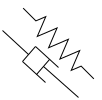
\includegraphics[width=0.6\textwidth]{Deplacement2D-1.png}
                \caption{Floe de glace 2D}
            \end{figure}

        }

        \mycol{60}{
            \myfig{PlotDeplacement2D-1-NonConv.png}{Simulation avec $T=10$}

            % \myfig{PositionInitFinales.png}{Illustration à $T=4$}
        }

    }

    Les équations de Newton-Euler :
    \begin{align*}
        \forall i \in \mathbb{Z}/3\mathbb{Z}+\{1\}, \quad m \ddot{\bvec{q}}_i = \sum_{j=i+1}^{i+2}C_{ij} \left[  k \left( \Vert \bvec{q}_j - \bvec{q}_i \Vert - L_{ij} \right) \bvec{u}_{ij} - \mu \left\langle \dot{\bvec{q}}_j - \dot{\bvec{q}}_i, \, \bvec{u}_{ij}  \right\rangle  \bvec{u}_{ij}  \right] . 
    \end{align*}

    Schéma d’Euler explicite :
    \begin{align*} \label{eq:systeme2D}
        \bvec{q}_{i}^{n+1} = 2\bvec{q}_{i}^{n}-\bvec{q}_{i}^{n-1} + \frac{\Delta t^2}{m} \sum_{j=i+1}^{i+2}C_{ij}\left[ k \left( \Vert \bvec{q}_j^n - \bvec{q}_i^n \Vert - L_{ij} \right) \bvec{u}_{ij} - \frac{\mu}{\Delta t} \left\langle \bvec{q}_{j}^{n}-\bvec{q}_{j}^{n-1} - \bvec{q}_{i}^{n}+\bvec{q}_{i}^{n-1}, \, \bvec{u}_{ij} \right\rangle  \bvec{u}_{ij}  \right].
    \end{align*}
    
\end{frame}


\begin{frame}[fragile]{Déplacement d'un floe isolé (2)}

    \tiny
    \begin{lstlisting}[language=Python,caption=Code de simulation et schéma avec Scipy]
                                    q0 = np.stack([q1_0, dotq1_0, q2_0, dotq2_0, q3_0, dotq3_0])
                                    q0_ = np.reshape(q0, (nb_nodes*4))

                                    def model(t, Q_):
                                        Q = np.reshape(Q_, (nb_nodes*2, 2))
                                        Q_ret = np.zeros_like(Q)
                                        Q_ret[2*0] = 0; Q_ret[2*1] = 0
                                        
                                        for i in range(1, nb_nodes):
                                            Q_ret[2*i] = Q[2*i+1] 
                                            
                                            for neighbor in range(i+1, i+3):
                                                j = neighbor % nb_nodes
                                                u[i,j] = (Q[2*j] - Q[2*i]) / nplin.norm(Q[2*j] - Q[2*i])
                                                Q_ret[2*i+1] += (1 / m)*C[i,j]*( k*(nplin.norm(Q[2*j]-Q[2*i]) - L[i,j])*u[i,j]
                                                                -  mu*(np.dot(Q[2*j+1] - Q[2*i+1], u[i,j]))*u[i,j] )
                                        return np.reshape(Q_ret, (nb_nodes*4))

                                    sol = solve_ivp(model, [0,T], q0_, t_eval=t)
    \end{lstlisting}

    \begin{figure}
        \centering
        \includegraphics[width=0.6\textwidth]{PositionInitFinales.png}
        \caption{Illustration à $T=4$}
    \end{figure}


\end{frame}